Las Estructuras Interactuables son estructuras que cuando un jugador se acerca a ella, son capaces de ser interactuadas.

\subsubsection{Portales}
Los portales son objetos colocables que permiten transportar al jugador 
de una ubicación a otra, ya sea dentro de la misma zona o entre zonas distintas de un mismo mundo. Cada portal 
se configura asociándolo a una zona de destino, de modo que, al interactuar con él, el jugador es teletransportado 
al punto configurado conservando su estado y progresión. De esta manera, los portales constituyen el mecanismo 
principal de conexión entre las distintas zonas que componen un mundo, permitiendo a los creadores diseñar mundos 
extensos y estructurar la navegación del jugador a través de ellos.

\begin{figure}[H]
\centering
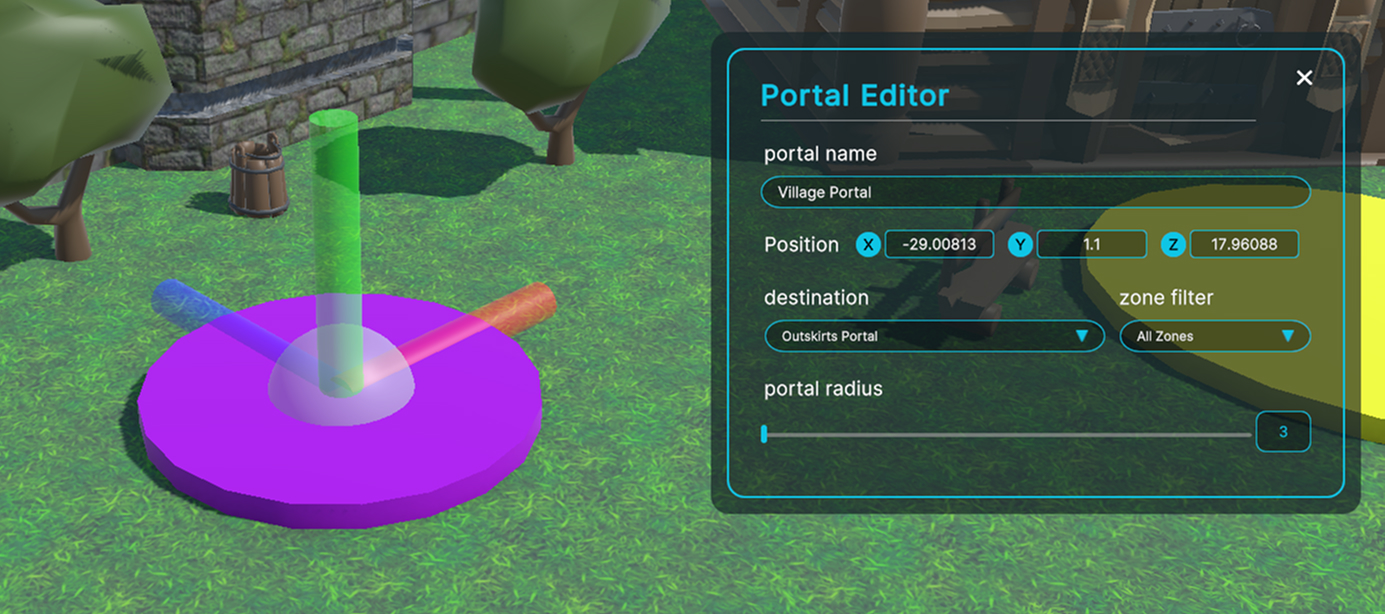
\includegraphics[width=0.85\textwidth]{img/08-implemented-solution/product/portal.jpg}
\caption{Portal colocado en la escena.}
\end{figure}

\begin{figure}[H]
\centering
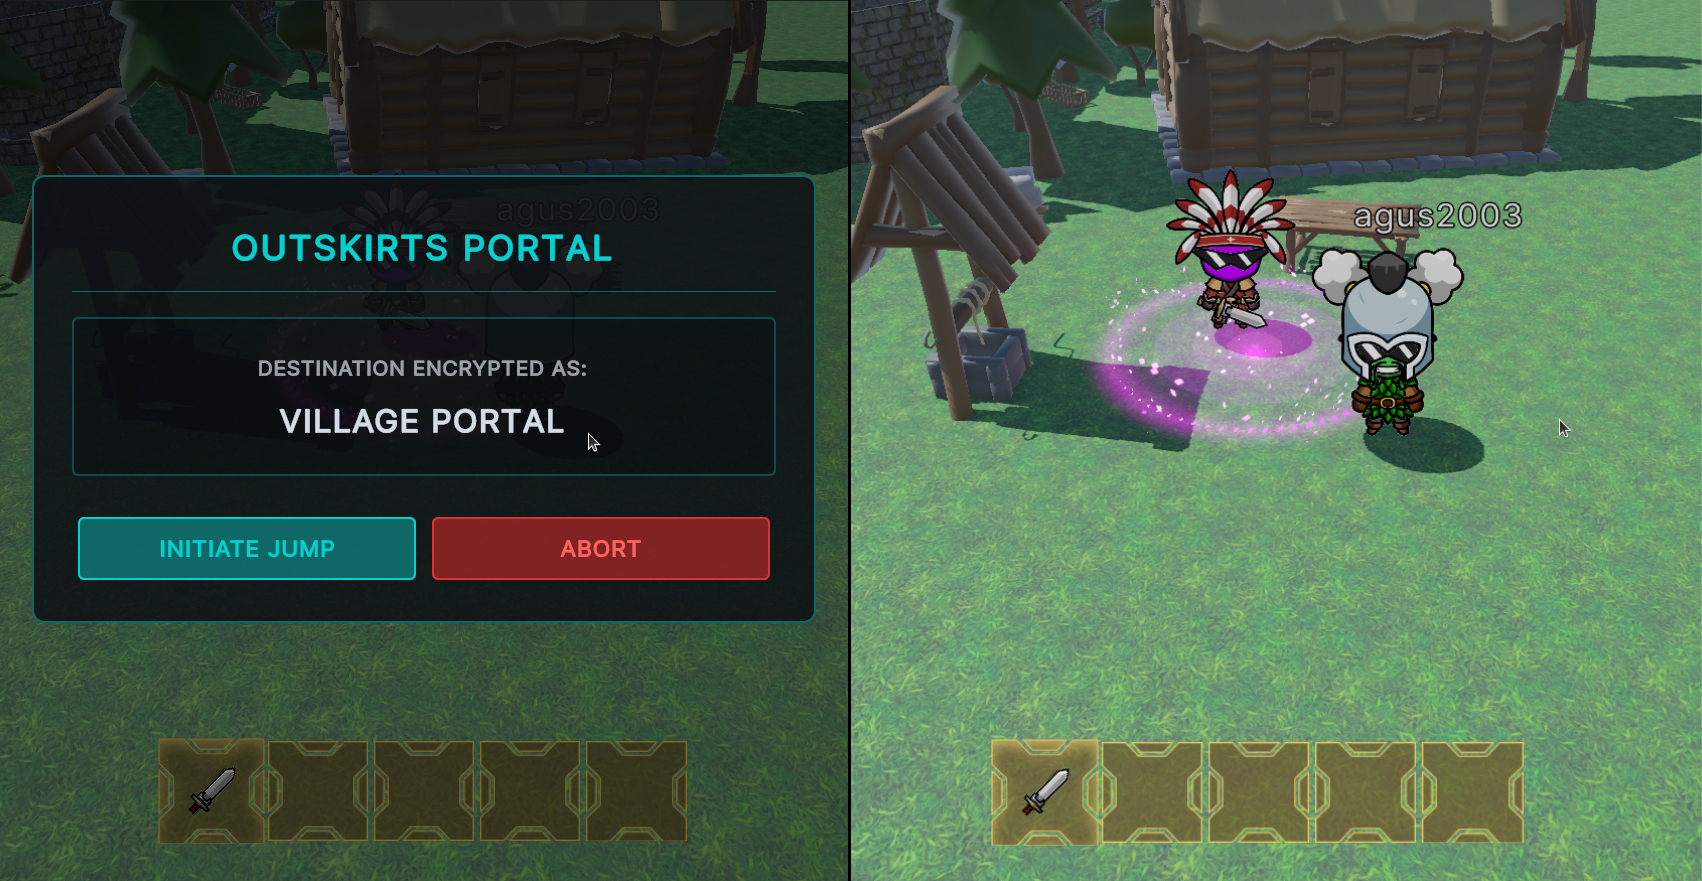
\includegraphics[width=0.75\textwidth]{img/08-implemented-solution/product/portals.jpg}
\caption{Captura de un jugador interactuando con un portal.}
\end{figure}

\subsubsection{Cofres}
Los cofres son objetos interactuables que los jugadores pueden abrir para obtener recompensas. Su botín 
(\textit{Loot Table}) puede configurarse de modo que, al abrir el cofre, se generen ítems de acuerdo con la 
configuración que se verá más adelante. Además, es posible definir un tiempo de reseteo, transcurrido el cual 
el cofre vuelve a estar disponible para abrirse nuevamente, lo que permite reutilizarlo como una fuente 
recurrente de recompensas. En cuanto a su apariencia, cada cofre admite una representación visual diferenciada 
para los estados abierto y cerrado, y permite seleccionar distintos modelos 3D, ya sea de la biblioteca de 
modelos predeterminados o de modelos personalizados importados por el creador. El modelo utilizado por defecto 
al colocar un cofre puede definirse desde el editor de modelos 3D.

\begin{figure}[H]
\centering
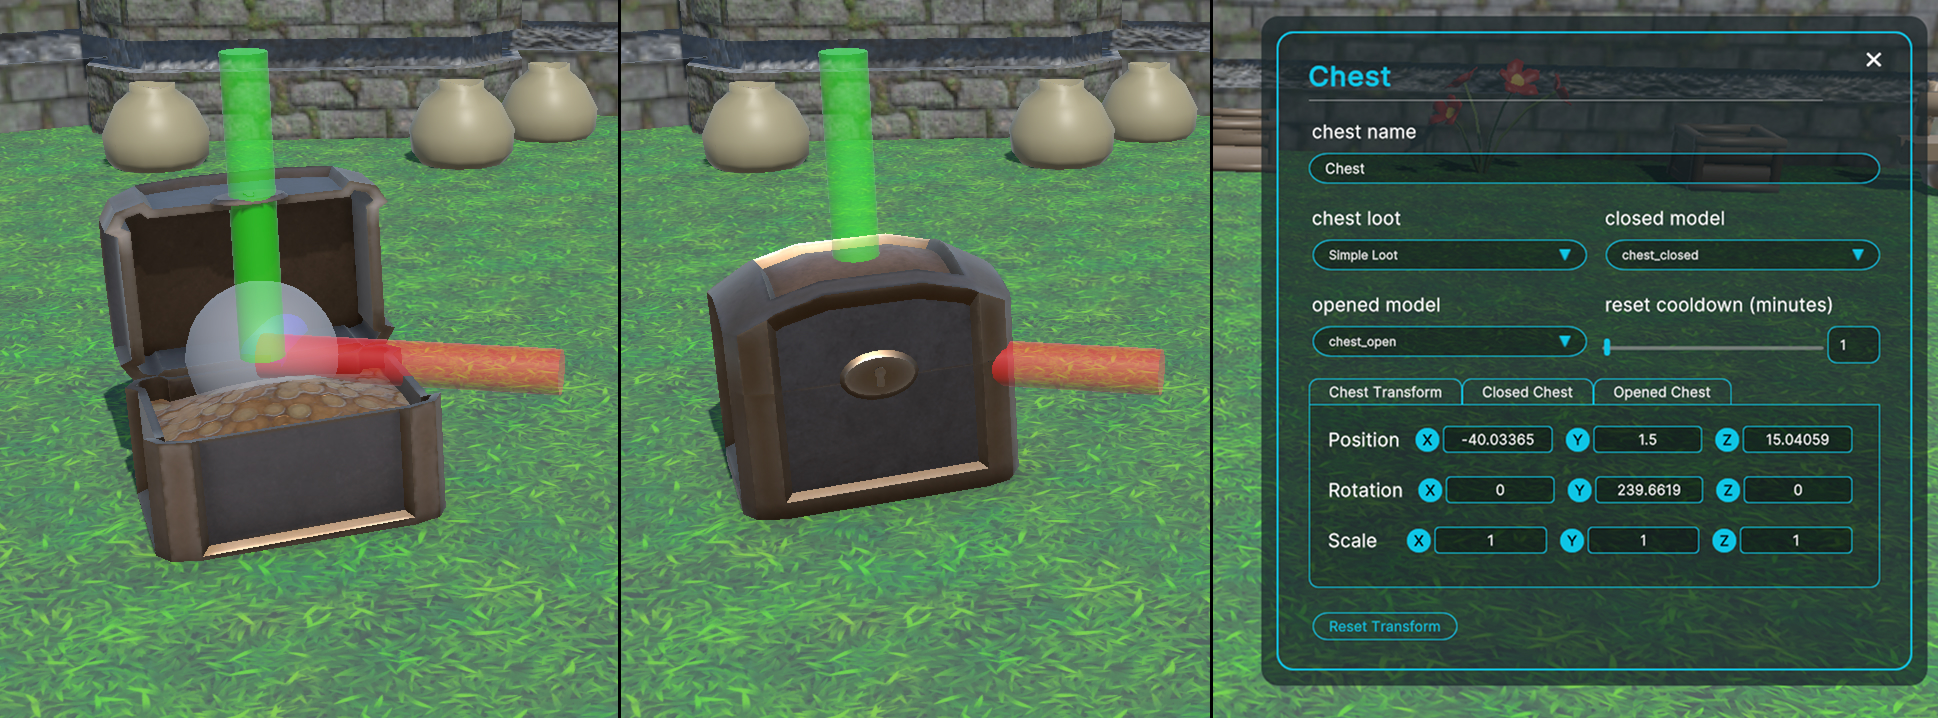
\includegraphics[width=\textwidth]{img/08-implemented-solution/product/chests.jpg}
\caption{Captura de cofres en el editor de mundos.}
\end{figure}

\begin{figure}[H]
\centering
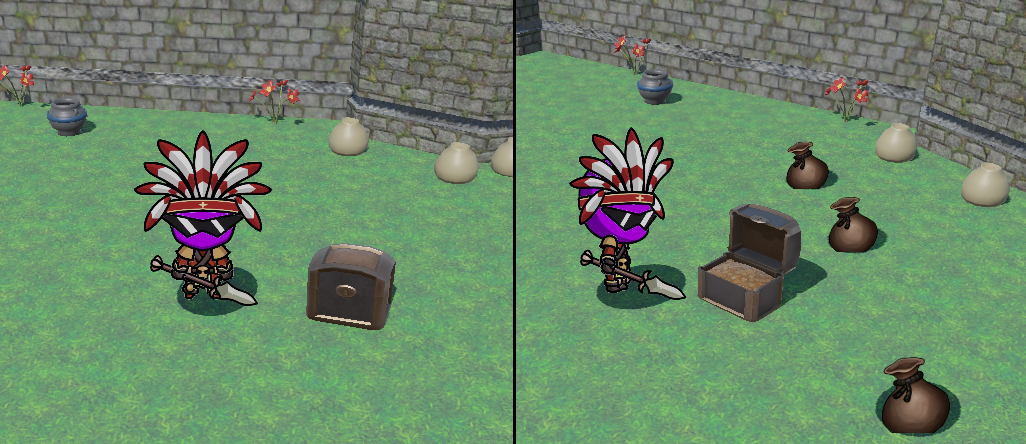
\includegraphics[width=0.75\textwidth]{img/08-implemented-solution/product/game-chest.jpg}
\caption{Captura de un jugador interactuando con un cofre.}
\end{figure}
